\documentclass[11pt]{article}   % tipo de documento e tamanho das letras

% os seguintes pacotes estendem a funcionalidade básica:
\usepackage[a4paper, total={16cm, 24cm}]{geometry} % tamanho da pagina e do texto
\usepackage[portuguese]{babel}  % traduz para portugues
\usepackage[utf8]{inputenc}
\usepackage{graphicx}           % graficos
\usepackage{amsmath}            % matematica
\usepackage{tikz}               % diagramas
    \usetikzlibrary{shadows}
\usepackage{booktabs}           % tabelas com  melhor aspecto
\usepackage[colorlinks=true]{hyperref}           % links para partes do documento ou para a web
\usepackage{listings}           % incluir codigo
    \renewcommand\lstlistingname{Listagem}  % Listing em portugues
    \lstset{numbers=left, numberstyle=\tiny, numbersep=5pt, basicstyle=\footnotesize\ttfamily, frame=tb,rulesepcolor=\color{gray}, breaklines=true}
\usepackage{blindtext}

% -------------------------------------------------------------------------------------------
\title
{
    
\includegraphics[width=0.3\textwidth]{images/logo_universidade.png}
    \\[0.1cm]
    \textbf{Simulador de Escalonamento de Processos} \\
    Sistemas Operativos I
}

\author
{
    \textbf{Professor:} Luís Rato \\
    \textbf{Realizado por:} Miguel de Carvalho 43108 
}
\date{3 de Abril de 2020}

% -------------------------------------------------------------------------------------------
%                                Body                                                       %
% -------------------------------------------------------------------------------------------

\begin{document}
\maketitle

% -------------------------------------------------------------------------------------------
\section{Introdução} 

\hspace{0,5cm}Neste trabalho foi solicitado a realização de um programa que simule o \textbf{Escalonamento de Processos} num modelo de 3 estados. Na figura abaixo está representado o diagrama que descreve o modelo de 3 estados:\par
\begin{figure}[h!]
    \begin{center}
        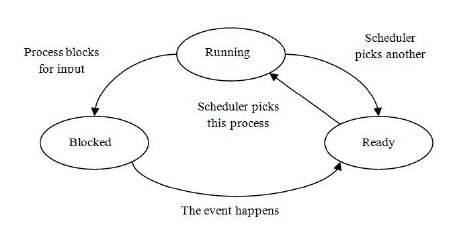
\includegraphics[width=0.5\textwidth]{images/states.png}
        \caption{Diagrama de 3 Estados}
    \end{center}
\end{figure}
O \textbf{Escalonador de Processos} faz parte do \textbf{Sistema Opertivo} e é responsável por decidir em que momento cada processo estará no CPU. 
Existem muitos algoritmos de escalonamento para realizar essa decisão. \par
Neste trabalho serão utilizados o algoritmo \textbf{FCFS} e o \textbf{Round Robin (RR)}:
\begin{itemize}
    \item O \textbf{FCFS} é um algoritmo de escalonamento não preemptivo que prioriza os processos pela ordem de chegada. Executa o processo todo do inicio ao fim sem o interromper, até estar concluído. Quando aparece um novo processo e ainda existe um em execução, esse novo irá para a fila de espera.
    \item O \textbf{Round Robin (RR)} é um algoritmo de escalonamento preemptivo que apresenta um funcionamento igual ao do \textbf{FCFS}, mas com tempo limite de execução, o \textbf{Quantum}. Ou seja, quando o processo se encontra em execução este irá ser interrompido quando o tempo de execução for igual ao /textbf{Quantum} e irá para a fila de espera (\textbf{READY}) 
\end{itemize}

% -------------------------------------------------------------------------------------------
\section{Implementação}

\hspace{0,5cm}Primeiramente comecei por pensar como deveria proceder para realizar o trabalho, na primeira tentativa comecei por desenvolver o \textbf{FCFS}, mas na segunda tentativa cheguei a conclusão de que não seria necessário realizar um programa para a implementação do \textbf{FCFS} e outro para o \textbf{Round Robin}, pois ambos são iguais, execto existir um limite de execução (\textbf{Quantum}) no \textbf{RR}.
Poderei então meter um \textbf{Quantum} muito grande e estarei perante o \textbf{FCFS}. \par
Comecei por proceder à criação das queues que iriam ser utilizados para guardar a informação de cada estado (\textbf{READY}, \textbf{RUN} e \textbf{BLOCKED}) e das respetivas funções essenciais para a sua manipulação. \par
O próximo desafio foi proceder a leitura do input (ficheiro com os processos e os tempos), para isso foi necessário proceder a criação de uma \textbf{Struct} para guardar a informação dos processos.
Através do \verb|fscanf| procedi a leitura do ficheiro e posteriormente permitiu guardar os processos na \textbf{Struct}. \par
Por conseguinte, comecei por desenvolver a função \newline
\verb|void scheduler(int n_process, process_t *process_arr[], int n_quantum)| que iria realizar as trocas dos processos entre os 3 estados. 
Esta função funciona de forma \textbf{cíclica}, ou seja a variável \textbf{i} corresponde ao \textbf{instante} em que o \textbf{escalonador} se encontra.
Este ciclo inicia em 0, que irá ser o instante inicial e termina quando todos os processos já tiverem sido executados.
Foi necessário também proceder a criação de novas funções para facilitar alguns procedimentos que eram realizados de forma repetitiva.
Demonstrou ser a função mais difícil de realizar devido a complexidade dos requísitos para os processos mudarem de estados. 
% -------------------------------------------------------------------------------------------
\section{Funções}
    
\begin{itemize}
    \item Funções pertencentes há manipulação das \verb|queues|:
        \begin{itemize}
            \item A função "\verb|queue_t *create_queue (int sz)|" cria a estrutura e aloca espaço para a \verb|queue|;
            \item A função "\verb|void insert (queue_t *queue, int element)|" adiciona elementos na stack;
            \item A função "\verb|bool full (queue_t *queue)|" verifica se a stack se encontra \textbf{cheia}. Caso esteja, devolve \verb|True|;
            \item A função "\verb|bool empty (queue_t *queue)|" verifica se a stack se encontra \textbf{vazia}. Caso esteja, devolve \verb|True|;
            \item A função "\verb|int get (queue_t *queue)|" remove o primeiro elemento da stack, dando \verb|return| desse valor e move os elementos para a esquerda \verb|queue|. Por exemplo o elemento da posição 2 passa para a posição 1;
            \item A função "\verb|void printQueue(queue_t *queue)|" dá \verb|print| de todos os elementos da \verb|queue|;
            \item A função "\verb|int top(queue_t *queue)|" dá \verb|return| do valor da última posição do \verb|queue|.
        \end{itemize}
    \item Funções pertencentes há manipulação da \verb|struct de processos|:
        \begin{itemize}
            \item A função "\verb|process_t *create_process(int sz);|" cria a estrutura e aloca espaço para o \verb|processo|;
            \item A função "\verb|process_t *insert_process(int beg, int end, int queues, int arr[]);|" \newline insere um processo;
            \item A função "\verb|int find_PID(int PID, process_t *process_arr[], int n_process)|" procura o PID no array e devolve a sua posição;
            \item A função "\verb|void update_run(int n_process, process_t *process_arr[])|" decrementa a primeira posição do run do processo;
            \item A função "\verb|void update_blocked(int n_process, process_t *process_arr[])|" decrementa a primeira posição do blocked do processo;
            \item A função "\verb|void update_index_run(int n_process, process_t *process_arr[], int size)|" \newline move os elementos do run do processo para a esquerda e verifique se existe algum número maior que 1000, caso exista irá mudar esse valor para 0;
            \item A função "\verb|void update_index_blocked(int n_process, process_t *process_arr[], int size)| \newline move os elementos do blocked do processo para a esquerda e verifique se existe algum número maior que 1000, caso exista irá mudar esse valor para 0"
        \end{itemize}
\end{itemize}

%-------------------------------------------------------------------------------------------
\section{Execução}

\hspace{0,5cm}Para executar o \textbf{Simulador de Escalonamento} o utilizador deverá passar como argumento, qual algoritmo deseja usar e o ficheiro de input.
\begin{itemize}
    \item Caso o utilizador escolha o \textbf{FCFS}, o \textbf{QUANTUM} irá ter um valor de \textbf{999}, assim nunca irá obrigar o programa a passar para o estado \textbf{READY}.
    \item Caso o utilizador escolha o \textbf{Round Robin}, o programa irá correr com o \text{Quantum} definido no código (\verb|#define QUANTUM_RR|).
\end{itemize}
% ----------\item ---------------------------------------------------------------------------------
\section{Análise de Resultados} % Conclusão
\begin{itemize}
    \item Escalonamento com o Algoritmo \textbf{FCFS}:
    \begin{itemize}
        \item Com o \verb|input1.txt|:
        \begin{verbatim}
Instant 0 - Ready: 101  | Run: 100 | Blocked: Empty!
Instant 1 - Ready: 200 300  | Run: 101 | Blocked: 100 
Instant 2 - Ready: 200 300  | Run: 101 | Blocked: 100 
Instant 3 - Ready: 200 300  | Run: 101 | Blocked: 100 
Instant 4 - Ready: 200 300 100  | Run: 101 | Blocked: Empty!
Instant 5 - Ready: 300 100  | Run: 200 | Blocked: 101 
Instant 6 - Ready: 300 100  | Run: 200 | Blocked: 101 
Instant 7 - Ready: 100  | Run: 300 | Blocked: 101 200 
Instant 8 - Ready: 100  | Run: 300 | Blocked: 101 200 
Instant 9 - Ready: 100 101  | Run: 300 | Blocked: 200 
Instant 10 - Ready: 100 101  | Run: 300 | Blocked: 200 
Instant 11 - Ready: 100 101  | Run: 300 | Blocked: 200 
Instant 12 - Ready: 100 101 200  | Run: 300 | Blocked: Empty!
Instant 13 - Ready: 100 101 200  | Run: 300 | Blocked: Empty!
Instant 14 - Ready: 101 200  | Run: 100 | Blocked: 300 
Instant 15 - Ready: 101 200  | Run: 100 | Blocked: 300 
Instant 16 - Ready: 101 200  | Run: 100 | Blocked: 300 
Instant 17 - Ready: 101 200  | Run: 100 | Blocked: 300 
Instant 18 - Ready: 101 200  | Run: 100 | Blocked: 300 
Instant 19 - Ready: 101 200  | Run: 100 | Blocked: 300 
Instant 20 - Ready: 101 200 300  | Run: 100 | Blocked: Empty!
Instant 21 - Ready: 101 200 300  | Run: 100 | Blocked: Empty!
Instant 22 - Ready: 101 200 300  | Run: 100 | Blocked: Empty!
Instant 23 - Ready: 101 200 300  | Run: 100 | Blocked: Empty!
Instant 24 - Ready: 200 300  | Run: 101 | Blocked: 100 
Instant 25 - Ready: 200 300  | Run: 101 | Blocked: 100 
Instant 26 - Ready: 300  | Run: 200 | Blocked: 100 
Instant 27 - Ready: 100  | Run: 300 | Blocked: 200 
Instant 28 - Ready: Empty! | Run: 100 | Blocked: 200 
Instant 29 - Ready: 200  | Run: 100 | Blocked: Empty!
Instant 30 - Ready: 200  | Run: 100 | Blocked: Empty!
Instant 31 - Ready: 200  | Run: 100 | Blocked: Empty!
Instant 32 - Ready: 200  | Run: 100 | Blocked: Empty!
Instant 33 - Ready: 200  | Run: 100 | Blocked: Empty!
Instant 34 - Ready: Empty! | Run: 200 | Blocked: Empty!
Instant 35 - Ready: Empty! | Run: 200 | Blocked: Empty!
Instant 36 - Ready: Empty! | Run: 200 | Blocked: Empty!    
    
        \end{verbatim}
    \end{itemize}
    \item Escalonamento com o Algoritmo \textbf{RR (Round Robin)}:
    \begin{itemize}
        \item Com o \verb|input1.txt|:
        \begin{verbatim}
Instant 0 - Ready: 101  | Run: 100 | Blocked: Empty!
Instant 1 - Ready: 200 300  | Run: 101 | Blocked: 100 
Instant 2 - Ready: 200 300  | Run: 101 | Blocked: 100 
Instant 3 - Ready: 200 300  | Run: 101 | Blocked: 100 
Instant 4 - Ready: 300 100 101  | Run: 200 | Blocked: Empty!
Instant 5 - Ready: 300 100 101  | Run: 200 | Blocked: Empty!
Instant 6 - Ready: 100 101  | Run: 300 | Blocked: 200 
Instant 7 - Ready: 100 101  | Run: 300 | Blocked: 200 
Instant 8 - Ready: 100 101  | Run: 300 | Blocked: 200 
Instant 9 - Ready: 101 300  | Run: 100 | Blocked: 200 
Instant 10 - Ready: 101 300  | Run: 100 | Blocked: 200 
Instant 11 - Ready: 101 300 200  | Run: 100 | Blocked: Empty!
Instant 12 - Ready: 300 200 100  | Run: 101 | Blocked: Empty!
Instant 13 - Ready: 200 100  | Run: 300 | Blocked: 101 
Instant 14 - Ready: 200 100  | Run: 300 | Blocked: 101 
Instant 15 - Ready: 200 100  | Run: 300 | Blocked: 101 
Instant 16 - Ready: 100 300  | Run: 200 | Blocked: 101 
Instant 17 - Ready: 300 101  | Run: 100 | Blocked: 200 
Instant 18 - Ready: 300 101  | Run: 100 | Blocked: 200 
Instant 19 - Ready: 300 101 200  | Run: 100 | Blocked: Empty!
Instant 20 - Ready: 101 200 100  | Run: 300 | Blocked: Empty!
Instant 21 - Ready: 200 100  | Run: 101 | Blocked: 300 
Instant 22 - Ready: 200 100  | Run: 101 | Blocked: 300 
Instant 23 - Ready: 100  | Run: 200 | Blocked: 300 
Instant 24 - Ready: 100  | Run: 200 | Blocked: 300 
Instant 25 - Ready: 100  | Run: 200 | Blocked: 300 
Instant 26 - Ready: Empty! | Run: 100 | Blocked: 300 
Instant 27 - Ready: 300  | Run: 100 | Blocked: Empty!
Instant 28 - Ready: 300  | Run: 100 | Blocked: Empty!
Instant 29 - Ready: 100  | Run: 300 | Blocked: Empty!
Instant 30 - Ready: Empty! | Run: 100 | Blocked: Empty!
Instant 31 - Ready: Empty! | Run: Empty!| Blocked: 100 
Instant 32 - Ready: Empty! | Run: Empty!| Blocked: 100 
Instant 33 - Ready: Empty! | Run: Empty!| Blocked: 100 
Instant 34 - Ready: Empty! | Run: 100 | Blocked: Empty!
Instant 35 - Ready: Empty! | Run: 100 | Blocked: Empty!
Instant 36 - Ready: Empty! | Run: 100 | Blocked: Empty!
Instant 37 - Ready: Empty! | Run: 100 | Blocked: Empty!
Instant 38 - Ready: Empty! | Run: 100 | Blocked: Empty!
Instant 39 - Ready: Empty! | Run: 100 | Blocked: Empty!            
        \end{verbatim}
    \end{itemize}
\end{itemize}

% -------------------------------------------------------------------------------------------
\section{Conclusão} % Conclusão
Em suma, este trabalho fez-me entender melhor como funciona o escalonador e as condições que cada algoritmo usa para proceder há mudança dos processos entre os estados e as diferenças de tempo. 
% -------------------------------------------------------------------------------------------
\end{document}